\documentclass[12pt]{article}		% use "amsart" instead of "article" for AMSLaTeX format
\usepackage[margin=1in]{geometry}	% See geometry.pdf to learn the layout options. There are lots.
\geometry{letterpaper}			% ... or a4paper or a5paper or ... 
%\geometry{landscape}                	% Activate for for rotated page geometry

\usepackage{amsmath}
\usepackage{amssymb}
\usepackage{amsthm}
\usepackage{amsbsy}
\usepackage{braket}
\usepackage{color}
\usepackage{dsfont}
\usepackage [english]{babel}
\usepackage{enumitem}
\usepackage{graphicx}			% Use pdf, png, jpg, or eps§ with pdflatex; use eps in DVI mode
							% TeX will automatically convert eps --> pdf in pdflatex
\usepackage{caption}
\usepackage{subcaption}

\usepackage{listings}
\usepackage{mathrsfs}
\usepackage [autostyle, english = american]{csquotes}
\usepackage{hyphenat}
\usepackage{hyperref}
\usepackage[parfill]{parskip}    		% Activate to begin paragraphs with an empty line rather than an indent
\usepackage{siunitx}
%\setlength{\parindent}{4em}
%\setlength{\parskip}{1em}

\MakeOuterQuote{"}

\title{Fokker-Planck equation and Heat equation with Crank-Nicolson Method}
\author{Akihiro Yamaguchi}
\date{Friday, December 16, 2016}			% Activate to display a given date or no date

\begin{document}
\maketitle
\begin{abstract}
This paper inspects numerical solutions of 1D heat equation (aka diffusion equation), 1D Fokker-Planck equation, and 2D heat equation with Crank-Nicolson (CN) method. Alternating direction implicit (ADI) method, one of the efficient CN methods for high dimensional (higher than 2D) space, is developed to compute numerical solutions of 2D heat equation. For comparison, a numerical solution of 2D heat equation is also computed with the simple explicit method.
\end{abstract}

\section*{Introduction}

% ================================================

\subsection*{Fokker-Planck equation and Heat equation}
The Fokker-Planck equation (also known as the Kolmogorov forward equation) is a parabolic partial differential equation that describes the time evolution of the probability density function. The equation is well-known for its use in Brownian motion, to study the probability density of the velocity of a particle under the influence of drag forces and random forces. However, this equation can also be generalized to many other systems, such as the probability density of the decision variable (a computational model of neurons in lateral intraparietal cortex known as the \textit{bounded accumulation model}) [1, 2].

According to Kiani and Shadlen [1], the propagation of the probability density of decision variable over time can be calculated using the Fokker-Planck equation given by:
\begin{equation} \label{eq:fp1d}
	\frac{\partial p(v,t)}{\partial t} = \left[- \frac{\partial \mu (v,t)}{\partial v} + \frac{\partial ^2}{\partial v^2} D(v,t) \right] p(v,t)
\end{equation}
where $D(v,t)$ is the diffusion coefficient ($D(v,t) > 0$) and $\mu (v,t)$ is the drift or advective coefficient. That is, the given equation is simplified to 
\[
	\frac{\partial p(v,t)}{\partial t} = -\mu \frac{\partial p(v,t)}{\partial v}   + D \frac{\partial ^2 p(v,t)}{\partial v^2}
\]
with $D(v,t) = 1$ and $\mu (v,t) = kc$, where $k$ is a constant given in Table 1 and $c$ is a motion strength that ranges from $0$ to $0.512$ (that corresponds to 0.0\% to 51.2\%) [1].

\begin{table}[h]
\begin{center}
    \begin{tabular}{ | l | l |}
    \hline
    k & 0.255 $\pm$ 0.002 \\ \hline
    B & 39.4 $\pm 10.0$ \\ \hline
    $\theta$ & $\pm$ 0.005  \\ \hline
    \end{tabular}
    \caption[Table caption text]{Fit parameters of the bounded accumulation model taken from [1].}
\end{center}
\end{table}

The boundary conditions of the Fokker-Planck equation are given by,
\begin{center}
$p(v, t_0) = \delta (v)$ and $p(\pm B, t) = 0$,
\end{center}
which enforce the constraints that the initial value of the decision variable is zero and that the accumulation terminates whenever the decision variable reaches one of the bounds ($\pm B$).

When $\mu = 0$, the given Fokker-Planck equation is equivalent to one-dimensional heat equation,
\[
	\frac{\partial u(x,t)}{\partial t} = D \frac{\partial u^2(x,t)}{\partial x^2}.
\]

% ================================================
In two dimensional case, the Fokker-Planck equation becomes:
\begin{equation} \label{eq:fp2d}
	\frac{\partial p(\vec{v},t)}{\partial t} = - \sum_{i=1}^{2} \mu_i \frac{\partial p(\vec{v},t)}{\partial v} + \sum_{i=1}^{2} \sum_{j=1}^{2} D_{ij} \frac{\partial^2 p(\vec{v},t)}{\partial v_i \partial v_j},
\end{equation}
where $p(\vec{v}, t)$ is the probability of the decision variable vector $\vec{v}$ at time $t$, and $D_{ij} = 0.5 \sum_{m=1}^{2} \sigma_{im} \sigma_{jm}$.

The boundary conditions of this 2D Fokker-Planck equation are given by 
\[
	p(\vec{v}, t_0) = \delta (v_1) \delta (v_2)
\]
and
\[
	p(v_i(t) = B_u, t) = 0,
\]
where $\delta(.)$ is the Kronecker delta function. 

The corresponding heat equation (for $\mu = 0$) is given by:
\[
	\frac{\partial u(x,y,t)}{\partial t} = D \left[ \frac{\partial u^2(x,y,t)}{\partial x^2} + \frac{\partial u^2(x,y,t)}{\partial y^2} \right].
\]

% ================================================
\newpage
\section*{Methodology}
Forward time centered space (FTCS) method (also known as Euler's method) is the most common method for solving the differential equations of the form 
\[
	\frac{d \phi}{dt} = \frac{D}{a^2}[\phi(x+a, t) + \phi(x-a,t) - 2\phi (x,t)],
\]
which gives us the solution by
\[
	\phi (x, t+h) = \phi (x,t) + h \frac{D}{a^2}[\phi(x+a, t) + \phi(x-a,t) - 2\phi (x,t)].
\]
For a given value of $\phi$ at every grid point $x$ at some time $t$, this equation tells us the value at every grid point at time $t+h$, a short time interval later. This equation provides us the solution to a partial differential equation (PDE).

This method works well for the diffusion equation but works less well in other forms of PDEs such as the wave equation because the calculation has become numerically unstable (errors dominate the calculation and the results). One possible approach to solve this stability problem is to use the implicit method. Moreover, the Crank-Nicolson (CN) method is also stable and more efficient than these explicit and implicit method.

Therefore, the CN method (a combination of the FTCS and the implicit method) is used to solve the 1D and 2D heat equation and 1D Fokker-Planck equation.

% ================================================

\subsection*{Crank-Nicolson method}
For a partial differential equation of the form
\[
	\frac{\partial u}{\partial t} = F \left( u, x, t, \frac{\partial u}{\partial x}, \frac{\partial^2 u}{\partial x^2}  \right),
\]
the Forward Euler method (or FTCS method) is given by
\[
	\frac{u^{n+1}_i - u^n_i}{\Delta t} = F^{n}_i \left(u, x, t, \frac{\partial u}{\partial x}, \frac{\partial^2 u}{\partial x^2} \right)
\]
and the Backward Euler method (or Implicit method) is given by
\[
	\frac{u^{n+1}_i - u^n_i}{\Delta t} = F^{n+1}_i \left(u, x, t, \frac{\partial u}{\partial x}, \frac{\partial^2 u}{\partial x^2} \right).
\]

By combining these two methods and taking an average, we obtain the CN method:
\[
	\frac{u^{n+1}_i - u^n_i}{\Delta t} = \frac{1}{2} [F^{n+1}_i \left(u, x, t, \frac{\partial u}{\partial x}, \frac{\partial^2 u}{\partial x^2} \right) + F^n_i \left(u, x, t, \frac{\partial u}{\partial x}, \frac{\partial^2 u}{\partial x^2} \right)].
\]

Since the CN method lies in between the FTCS and implicit methods, these equations are indirect (do not provide us an explicit expression), but can be solved as a set of simultaneous equations to provide us stable solution.

% ================================================

\subsection*{Crank-Nicolson (CN) method for Fokker-Planck Equation}
For the 1D bounded accumulation model, we study Eq. \eqref{eq:fp1d} given by 
\[
	\frac{\partial p(v,t)}{\partial t} = \left[- \frac{\partial \mu (v,t)}{\partial v} + \frac{\partial ^2}{\partial v^2} D(v,t) \right] p(v,t)
\]
with the boundary condition of 
\[
	\frac{\partial p}{\partial v} \bigg\rvert _{v = -B, B} = 0
\]
where $p$ is the probability density of decision variable, $D$ is the diffusion coefficient, $\mu$ is the drift or advective coefficient, and $B$ is the length of our one-dimensional space domain.

The CN Stencil is defined by
\[
	\frac{\partial p}{\partial t} \bigg\rvert _{v=j \Delta v, t = n\Delta t} \approx \frac{U_j^{n+1} - U_j^n}{\Delta t}
\]
The spatial part of the CN stencil for the second partial derivative term approximates the Laplace operator of the equation and takes the form:
\[
	\frac{\partial^2 p}{\partial v^2} \bigg\rvert _{v=j \Delta v, t = n\Delta t} \approx \frac{1}{2 \Delta v^2} \left(U_{j+1}^{n} - 2U_j^n + U_{j-1}^{n+1} + U_j^{n+1} - 2 U_j^{n+1}+ U_{j-1}^{n+1} \right)
\]
The CN stencil for the advection term is given by:
\[
	\mu \frac{\partial p}{\partial v} \approx \frac{\mu}{4 \Delta v} \left(U_{j+1}^{n} - U_{j-1}^n + U_{j+1}^{n+1} - U_{j-1}^{n+1} \right)
\]

Applying this stencil to grid point ${(j,n)}$  gives the following approximation of the equation:
\[
	\frac{U_{j}^{n+1} - U_j^{n}}{\Delta t} = \frac{D}{2 \Delta v^2} \left(U_{j+1}^{n} - 2U_j^n + U_{j-1}^{n+1} + U_j^{n+1} - 2 U_j^{n+1}+ U_{j-1}^{n+1} \right) + \left(U_{j+1}^{n} - U_{j-1}^n + U_{j+1}^{n+1} - U_{j-1}^{n+1} \right).
\]
By replacing $\sigma = \frac{D \Delta t}{2 \Delta v^2}$ and $\rho = \frac{\mu \Delta t}{4 \Delta v}$ and rearranging the above approximation, we obtain:
\[
	(1+2 \sigma) U_j^{n+1} - (\sigma + \rho) U_{j+1}^{n+1} - (\sigma - \rho) U_{j-1}^{n+1} = (1-2\sigma) U_j^n + (\sigma + \rho)U_{j+1}^n + (\sigma-\rho) U_{j-1}^n
\]
for all grid points with spatial indices $j = 1, 2, ..., J-3, J -2$. On the two boundaries of our spatial grid, apply the above Neumann boundary conditions that dictate $U_{-1}^n = U_0^n$ and $U_{J-1}^n = U_J^n$ for $(n = 0, 1, ..., t_f)$.\\

In a vector and matrix form, this equation is given by:
\[
	\textbf{A} \textbf{U}^{n+1} = \textbf{B} \textbf{U}^n
\]

where
\begin{equation*} % \label{eq:matrix1}
	\textbf{U}^{n+1} = \begin{bmatrix} U_0^{n+1}\\ U_1^{n+1} \\ \vdots \\ U_{J-1}^{n+1} \end{bmatrix}, 
	\textbf{U}^n = \begin{bmatrix} U_0^n\\ U_1^n \\ \vdots \\ U_{J-1}^n \end{bmatrix},
\end{equation*}

\begin{equation*} % \label{eq:matrix1}
	\textbf{A} = 
	\begin{bmatrix} 
	1 + \sigma + \rho & - (\sigma + \rho) & 0 & \hdots & 0 & 0 \\ 
	- \sigma + \rho & 1 + 2 \sigma & - (\sigma + \rho) & \hdots & 0 & 0\\
	0 & - \sigma + \rho & 1 + 2 \sigma & \hdots & 0 & 0 \\
	\vdots & \vdots & \vdots & \ddots & \vdots & \vdots\\
	0 & \hdots & 0 & - \sigma + \rho & 1+2\sigma & - (\sigma + \rho) \\
	0 & \hdots & 0 & 0 & - \sigma + \rho & 1 + \sigma - \rho
	\end{bmatrix},
\end{equation*}
and 
\begin{equation*}
	\textbf{B} = 
	\begin{bmatrix}
	1 - \sigma - \rho & \sigma + \rho & 0 & \hdots & 0 & 0 \\ 
	\sigma -\rho & 1 - 2 \sigma & \sigma +\rho & \hdots & 0 & 0\\
	0 & \sigma -\rho & 1 - 2 \sigma & \hdots & 0 & 0 \\
	\vdots & \vdots & \vdots & \ddots & \vdots & \vdots\\
	0 & \hdots & 0 & \sigma -\rho & 1- 2\sigma & \sigma +\rho \\
	0 & \hdots & 0 & 0 & \sigma -\rho & 1 - \sigma + \rho
	\end{bmatrix}.
\end{equation*} 

Therefore, solving the linear equation gives the solution, as
\[
		\textbf{U}^{n+1} = \textbf{A}^{-1} \textbf{B} \textbf{U}^n.
\]

% ===============================================================
\subsection*{Simple explicit method for the 2D Heat equation}
One of the simplest method to compute numerical solution of the 2D heat equation is the explicit method.

With this scheme, by discretizing the terms of the 2D heat equation, we obtain:
\begin{align*}
	\frac{U_{j,k}^{n+1} - U_{j,k}^{n}}{\Delta t} =  \frac{U_{j+1,k}^{n} - 2 U_{j,k}^{n}+ U_{j-1,k}^{n}}{\Delta x^2} + \frac{U_{j,k+1}^{n} - 2 U_{j,k}^{n}+ U_{j,k-1}^{n}}{\Delta y^2}.
\end{align*}

This is equivalent to
\begin{equation*}
	U_{j,k}^{n+1} =  \frac{\Delta t}{\Delta x^2} \left(U_{j+1,k}^{n} - 2 U_{j,k}^{n}+ U_{j-1,k}^{n} \right) + \frac{\Delta t}{\Delta y^2} \left(U_{j,k+1}^{n} - 2 U_{j,k}^{n}+ U_{j,k-1}^{n} \right)
\end{equation*}
For $\Delta x = \Delta y$ and $r = \frac{\Delta t}{\Delta x^2}$, we get
\begin{equation*}
	U_{j,k}^{n+1} =  (1-4r) U_{j,k}^{n} + r \left(U_{j+1,k}^{n} + U_{j-1,k}^{n} + U_{j,k+1}^{n} + U_{j,k-1}^{n} \right).
\end{equation*}

This is very straightforward to implement. However, as it was mentioned earlier, this method is unstable for a small time-step. \\
The stability condition for this method is defined by $r \leq \frac{1}{2}$, where $r = \frac{\Delta t}{\Delta x^2}$, and $\Delta t$ will become very large (and it takes very long time to compute) to obtain a stable solution. Therefore, it is necessary to consider Crank-Nicolson method for a large number of grids (i.e., $N > 10$).

% ================================================

\subsection*{Crank-Nicolson method in 2D PDEs}
In 2D case, a naive generalization of CN scheme for 2D heat equation gives the form of
\begin{align*}
	\frac{U_{j,k}^{n+1} - U_{j,k}^{n}}{\Delta t} = & \frac{D}{2 \Delta x^2} \left(U_{j+1,k}^{n} - 2U_{j,k}^n + U_{j-1,k}^{n+1} + U_{j,k}^{n+1} - 2 U_{j,k}^{n+1}+ U_{j-1,k}^{n+1} \right) \\
	& + \frac{D}{2 \Delta y^2} \left(U_{j, k+1}^{n} - 2U_j^n + U_{j, k-1}^{n+1} + U_{j,k}^{n+1} - 2 U_{j,k}^{n+1}+ U_{j,k-1}^{n+1} .\right) 
\end{align*}

By making this into matrix form (for $\Delta x = \Delta y$ and $r = \frac{D \Delta t}{2 \Delta x^2}$) we get
\begin{align} \label{eq:cd2d}
	& (1+ 2r) U_{j,k}^{n+1} - \frac{r}{2} \left(U_{j+1,k}^{n+1} + U_{j-1,k}^{n+1} \right) - \frac{r}{2} \left(U_{j,k+1}^{n+1} + U_{j,k-1}^{n+1} \right) \\
	& = (1- 2r) U_{j,k}^{n} + \frac{r}{2} \left(U_{j+1,k}^{n} + U_{j-1,k}^{n} \right) + \frac{r}{2} \left(U_{j,k+1}^{n} + U_{j,k-1}^{n} \right) 
\end{align}
and
\[
	\textbf{A} \textbf{U}^{n+1} = \textbf{B} \textbf{U}^n
\]

where
\begin{equation*} % \label{eq:matrix1}
	\textbf{U}_{;, k}^{n+1} = \begin{bmatrix} U_{0,k}^{n+1}\\ U_{1,;}^{n+1} \\ \vdots \\ U_{J-1,k}^{n+1} \end{bmatrix}, 
	\textbf{U}_{;,k}^n = \begin{bmatrix} U_{0,k}^n\\ U_{1,k}^n \\ \vdots \\ U_{J-1,k}^n \end{bmatrix}.
\end{equation*}
This scheme is computationally inefficient because the matrix $\textbf{A}$ is block-tridiagonal (not tridiagonal) and inverting such matrix requires $O(JK)^2$ operations, where $J$ and $K$ corresponds to number of stencils in $x$ and $y$, respectively, and $O$ stands for the $(JK) \times (JK)$ zero matrix. However, the Alternating Direction Implicit (ADI) method utilizes tridiagonal matrices instead of block-tridiagonal, and is a computationally efficient scheme.

% ===============================================================

\subsection*{CN and Altering Direction Implicit (ADI) method for 2D PDE}
In order to solve the 2D FP and heat equation, it is possible to generalize the CN method. However, a naive generalization of the CN method, given by 
\[
		U_{j,k}^{n+1} = U_{j,k}^{n} + \frac{r}{2} (\delta^2_x + \delta^2_y) \left(U_{j,k}^n + U_{j,k}^{n+1} \right),
\]
where $\delta^2_x$ and $\delta^2_y$ are matrices to simplify Eq. [3, 4], is computationally inefficient. Therefore, it is necessary to adopt equally accurate and stable but more efficient method.

A scheme that satisfies such conditions is called \textit{Altering Direction Implicit (ADI)} method. 

The ADI method can be implemented using
\[
	\left(1- \frac{r}{2}\delta^2_x \right) \left(1- \frac{r}{2}\delta^2_y \right) U_{j,k}^{n+1} =\left(1 +  \frac{r}{2}\delta^2_x \right) \left( 1+\frac{r}{2}\delta^2_y \right) U_{j,k}^n,
\]
in a two-step method, which is given by:
\begin{align*}
	&(1): \left(1- \frac{r}{2}\delta^2_x \right) U^{n+1/2}_{j,k} = \left( 1+\frac{r}{2}\delta^2_y \right) U_{j,k}^n, \\
	&(2): \left(1- \frac{r}{2}\delta^2_y \right) U_{j,k}^{n+1} = \left( 1+\frac{r}{2}\delta^2_x \right) U^{n+1/2}_{j,k}.
\end{align*}

In more detail, the steps to implement this method is as follows: \\
\textbf{Step 1}:
\begin{equation*}
	\left(1- \frac{r}{2}\delta^2_x \right) \vec{\textbf{U}}^{n+1/2}_{;,k} = \vec{\textbf{U}}_{;,k}^n + \frac{r}{2} \left(\vec{\textbf{U}}_{;,k+1}^n - 2 \vec {\textbf{U}}_{;,k}^n + \vec{\textbf{U}}_{;,k-1}^n \right) + \frac{r}{2} \vec{b}'_{;,k} \\
\end{equation*}
where $\frac{r}{2} \delta_x^2$ is an $(J-1)\times (J-1)$ matrix, with 
\begin{equation*}
	\vec{\textbf{U}}^{n+1/2}_{;,k} = \begin{bmatrix} U^{n+1/2}_{1,k} \\ U^{n+1/2}_{2,k} \\ \vdots \\ U^{n+1/2}_{J-2,k} \\ U^{n+1/2}_{J-1,k} \end{bmatrix}, 
	\vec{\textbf{U}}_{;,k}^{n} = \begin{bmatrix} U_{1,k}^{n} \\ U_{2,k}^{n} \\ \vdots \\ U_{J-2,k}^{n} \\ U_{J-1,k}^{n} \end{bmatrix}, 
	\vec{\textbf{b}}'_{;,k} = \begin{bmatrix} g_{top, k} \\ 0 \\ \vdots \\ 0 \\ g_{bottom, k} \end{bmatrix}.
\end{equation*} 


\textbf{Step 2}:
\begin{equation*}
	\left(1- \frac{r}{2}\delta^2_y \right) \vec{\textbf{U}}_{j,;}^{n+1} = \vec{\textbf{U}}_{j,;}^{n+1/2} + \frac{r}{2} \left(\vec{\textbf{U}}_{j+1,;}^{n+1/2} - 2 \vec {\textbf{U}}_{j,;}^{n+1/2} + \vec{\textbf{U}}_{j-1,;}^{n+1/2} \right) + \frac{r}{2} \vec{b}_{j,;} \\
\end{equation*}
where $\frac{r}{2} \delta_y^2$ is an $(K-1)\times (K-1)$ matrix, with 
\begin{equation*}
	\vec{\textbf{U}}^{n+1}_{j,;} = \begin{bmatrix} U^{n+1}_{j,1} \\ U^{n+1}_{j,2} \\ \vdots \\ U^{n+1}_{j,K-2} \\ U^{n+1}_{j,K-1} \end{bmatrix}, 
	\vec{\textbf{U}}_{j,;}^{n+1/2} = \begin{bmatrix} U_{j,1}^{n+1/2} \\ U_{j,2}^{n+1/2} \\ \vdots \\ U_{j,K-2}^{n+1/2} \\ U_{j,K-1}^{n+1/2} \end{bmatrix}, 
	\vec{\textbf{b}}_{j,;} = \begin{bmatrix} g_{j, right} \\ 0 \\ \vdots \\ 0 \\ g_{j, left} \end{bmatrix}.
\end{equation*} 

In both step 1 and 2, the matrices defined by $1-\frac{r}{2} \delta x^2$ and $1-\frac{r}{2} \delta y^2$ in the left hand side are tridiagonal, and the inverse of these matrices can be easily made.

% ================================================
\newpage
\section*{Results and Discussion}
This section describes the results obtained by the aforementioned methods (i.e., Explicit method, Crank Nicolson method, and Alternating Direction Implicit method) and discusses the error convergence rate of 1D heat equation for the CN method. Qualitative analyses of 1D Fokker-Planck equation and  2D heat equation are also described.

\subsection*{1D Heat Equation}
The heat diffusion with the initial condition defined by Dirac-delta function in a 1D domain is plotted in Fig. 1. The initial condition is defined by $\delta (x-0.005)$ with $D = 4.25 \times 10^{-6}$.

\begin{figure}[h]
\centering
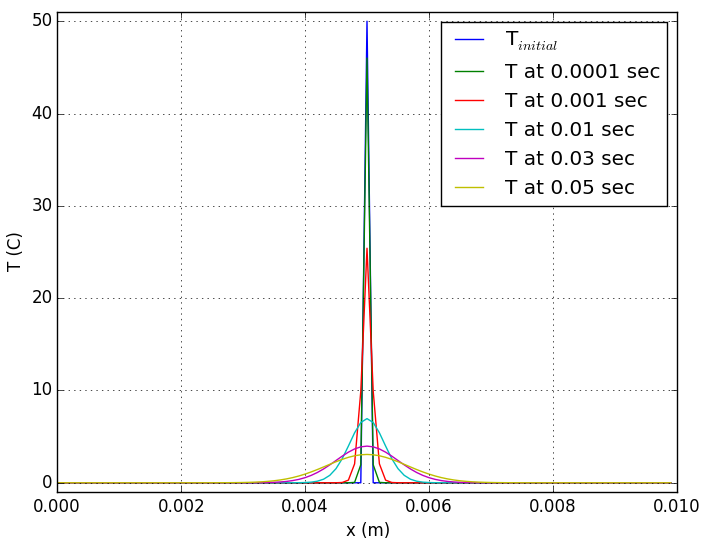
\includegraphics[height=6cm]{figure-1-1d_heat.png}\quad
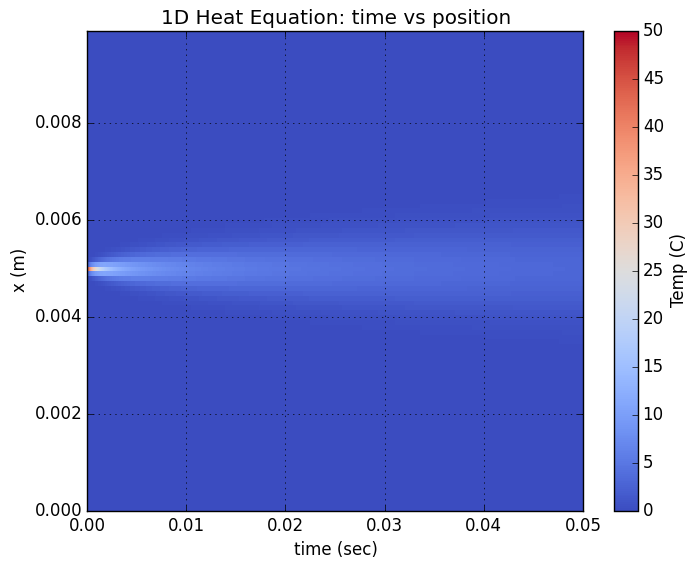
\includegraphics[height=6cm]{figure-2-1d_heat.png}\par\medskip
\caption{CN method for 1D heat equation. (\textbf{left}) position vs. temperature. The initial condition is defined by a Dirac-delta function with $T = \SI{50}{\degreeCelsius}$ at $x = 0.005$. (\textbf{right}) time vs. position. Time evolution of a 1D heat for $t = 0 sec$ to $t = 0.05 sec$.}

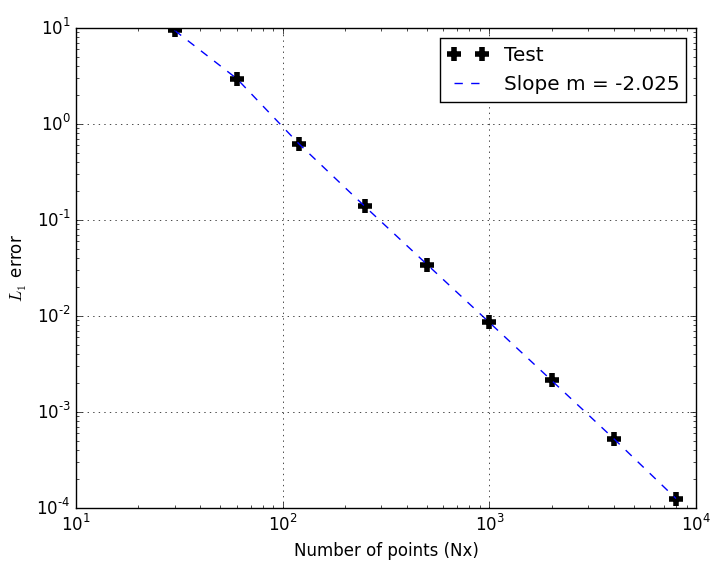
\includegraphics[scale=0.4]{figure-3_conv.png}
\caption{Error convergence plot for 1D heat equation with Crank Nicolson method. The grid number ($N_x$) ranges from $30$ to $8000$, and the slope of the convergence is around 2.0, which agrees with theoretically expected second order of accuracy.}
\end{figure}
The exact solution for the 1-d heat equation is given by a gaussian function:
\[
	T(x,t) = \sqrt{\frac{t_0}{t}} \exp{\frac{-x^2}{4 D t}},
\]
where $t_0$ is the initial height of the Dirac delta function and $D$ is the diffusion coefficient.

It is reasonable to expect that as the number of grid ($N_x$) increases at fixed $\delta t$, the accuracy of the numerical solution increases (i.e., the spatial resolution increases at fixed temporal resolution). This is what is shown in Fig. 2, the convergence of error in comparison with the analytic and numerical solutions for calculations performed with $D=4.25\times 10^{-6}$, $x_0 = 0.005$, $t_0=0.0$, $\delta t = 0.05$, and $N_x = 30$ to 8000. 


\newpage
\subsection*{1D Fokker-Planck Equation}
Using the same Crank Nicolson method as in 1D heat equation (with a slightly modified code for Eqn.1) with the initial conditions ($p(v, t_0) = \delta (v)$ and p$(\pm B, t) = 0$), Figure 3 and 4 (left) shows qualitatively equivalent diffusion of probability density as in Ref [1] (Fig. 4 (right)). 
\begin{figure}[h]
\centering
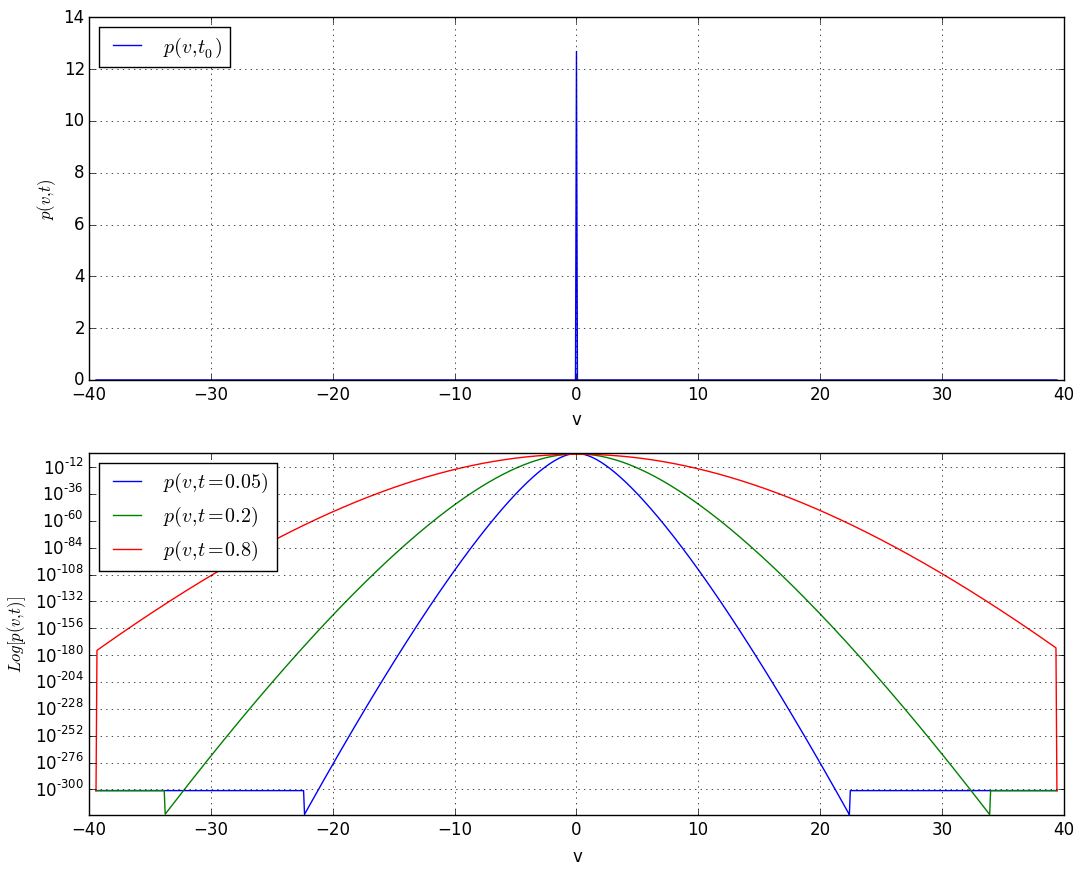
\includegraphics[height=8cm]{figure-4-1d_planck.png}\par\medskip
\caption{Decision variable ($v$) vs probability density of decision variable ($p(v,t)$). 
\\ (\textbf{top}) Initial condition defined by Dirac-delta function. (\textbf{bottom}) time evolution of a 1D delta function over time.}
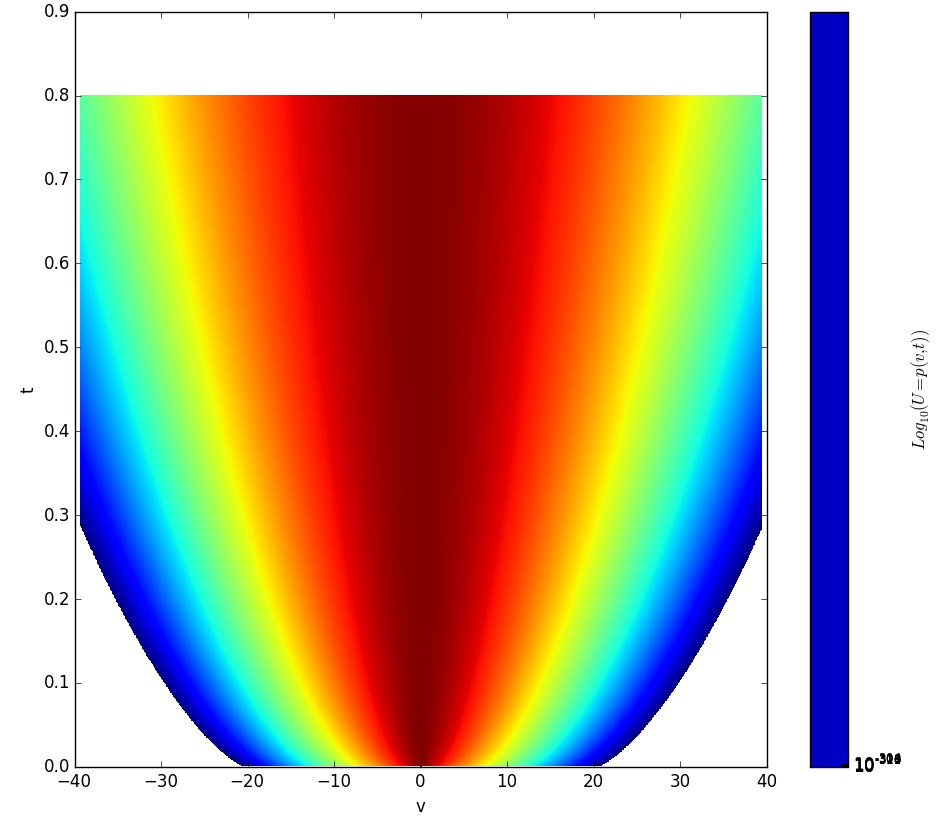
\includegraphics[height=5cm]{figure-5-1d_planck.png}\quad
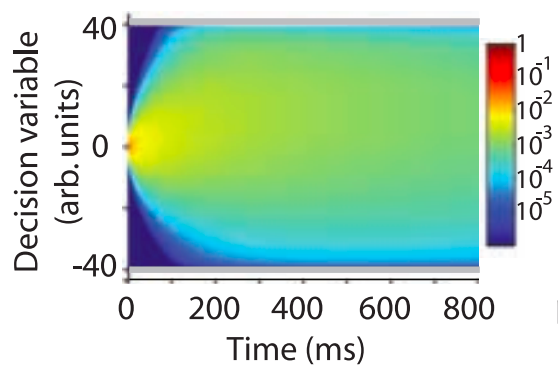
\includegraphics[height=5cm]{figure_ref1.png}
\caption{1D Fokker-Planck equation with Crank Nicolson method. (\textbf{left}) numerical solution of Fokker-Planck equation computed with ADI method over time ($v(t)$ vs $t$ with $p(v,t)$ in color). (\textbf{right}) numerical solution of Fokker-Planck equation from Ref [1] ($t$ vs $v(t)$)}
\end{figure}
\subsection*{2D Heat Equation}

\begin{figure}
\centering
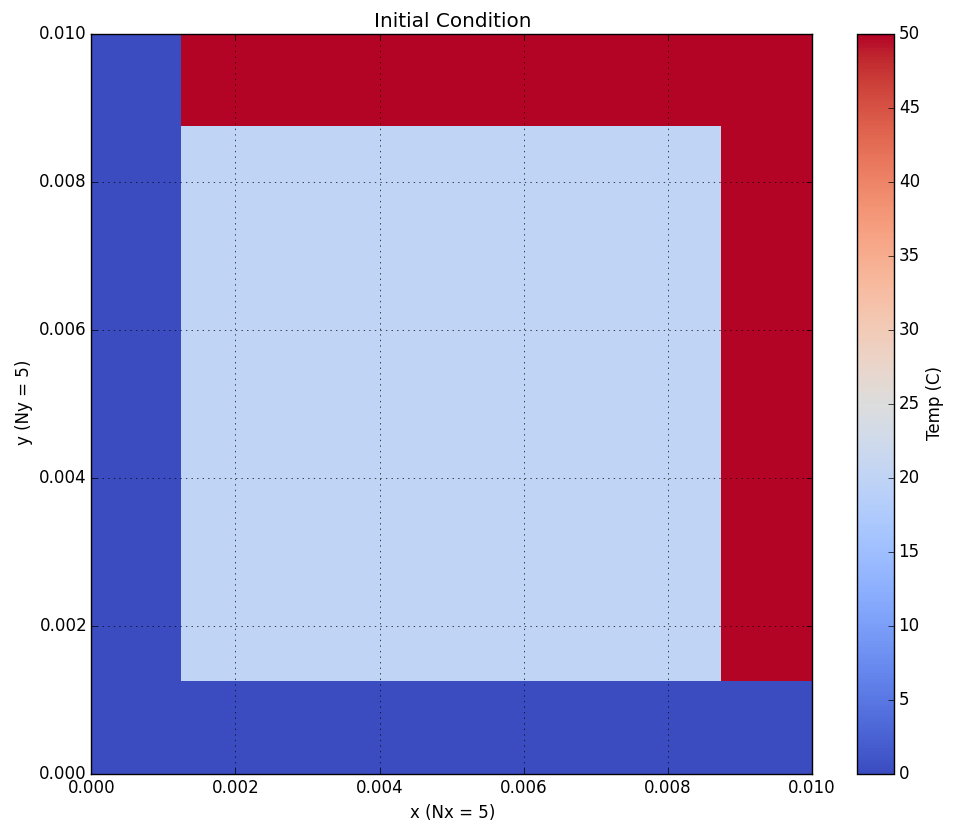
\includegraphics[height=6.5cm]{figure-6-2d_heat_init.png}\par\medskip
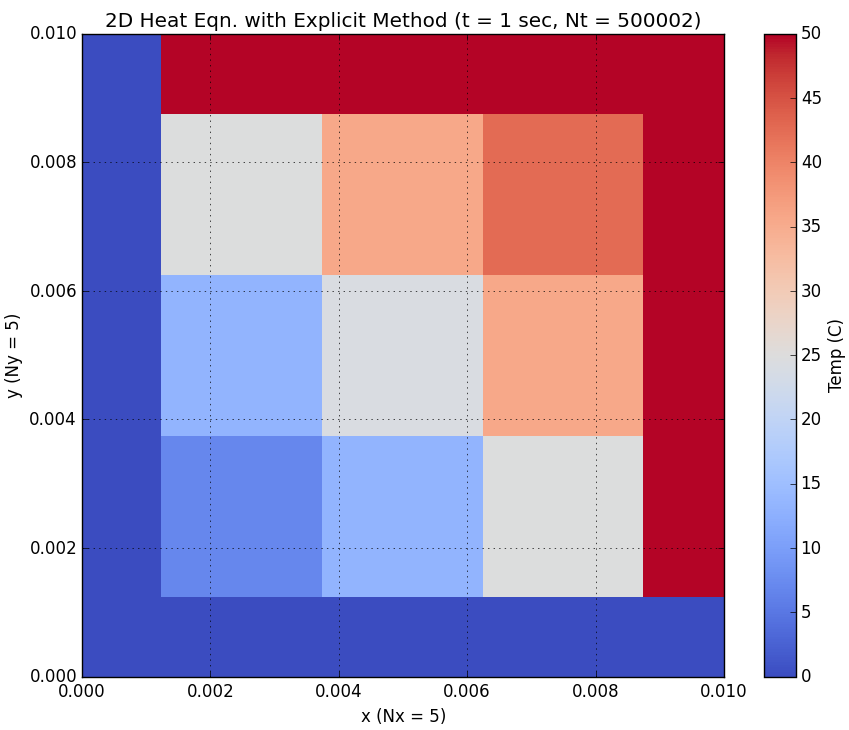
\includegraphics[height=6.5cm]{figure-7-2d_heat_exp.png}\quad
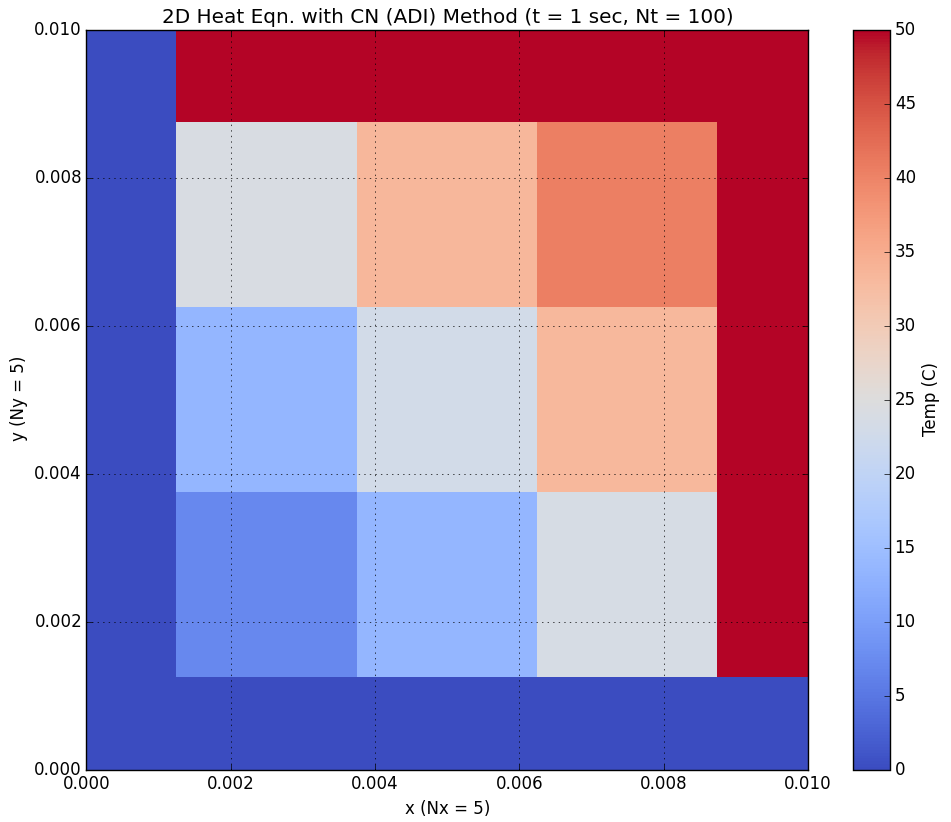
\includegraphics[height=6.5cm]{figure-8-2d_heat_adi.png}
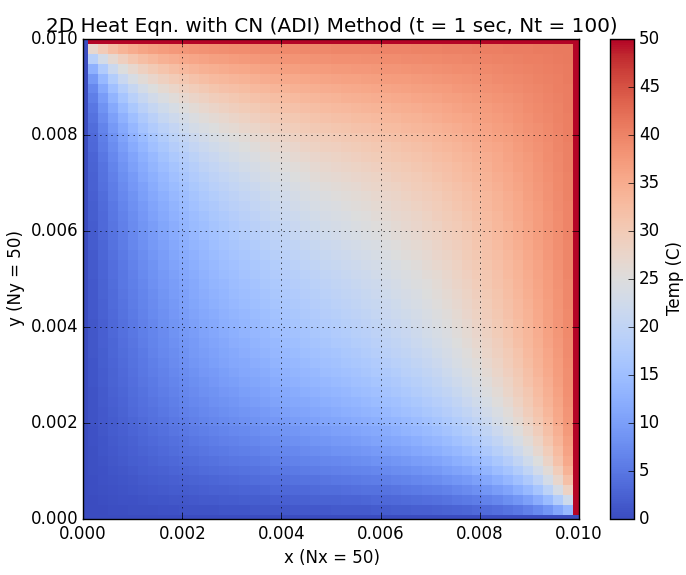
\includegraphics[height=6.5cm]{figure-10-2d_heat50.png}
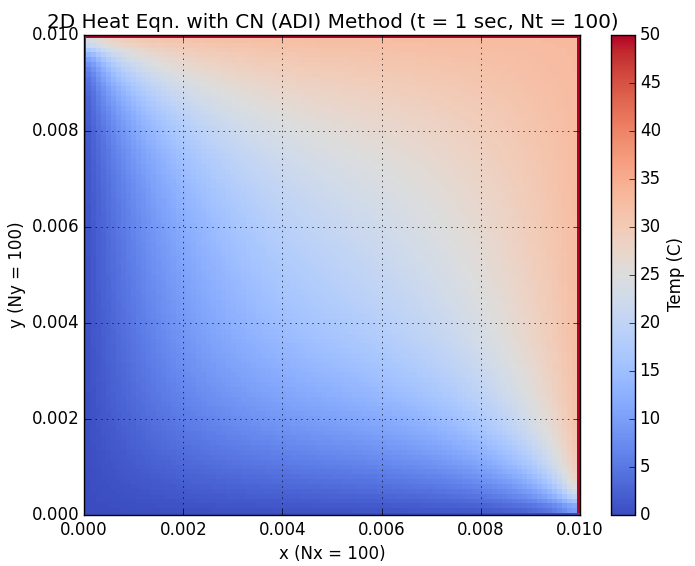
\includegraphics[height=6.5cm]{figure-11-2d_heat100.png}
\caption{Numerical solution of 2D heat equation. (\textbf{top}) Initial condition. (\textbf{middle left}) at $t = 1 sec$ with Explicit method and (\textbf{middle right}) Crank Nicolson method.
(\textbf{bottom left}) Temperature distribution at $t = 1 sec$ (CN method) with $N_x \times N_y = 50 \times 50$ and (\textbf{bottom right}) $N_x \times N_y = 100 \times 100$.}
\end{figure}

Figure 5 in the previous page inspects the numerical solution of the 2D heat equation (for $N_x \times N_y$ grids). The initial and boundary conditions are defined by high temperature (in red, ($\SI{50}{\degreeCelsius}$ at top and right edges) and low temperature (in dark blue, $\SI{0}{\degreeCelsius}$ at left and bottom edges) with variable middle temperature (in light blue, $\SI{20}{\degreeCelsius}$ center region).

All four plots qualitatively agrees with the expected temperature gradient in a squared domain. 

%\begin{figure}[h]
%	\centering
%	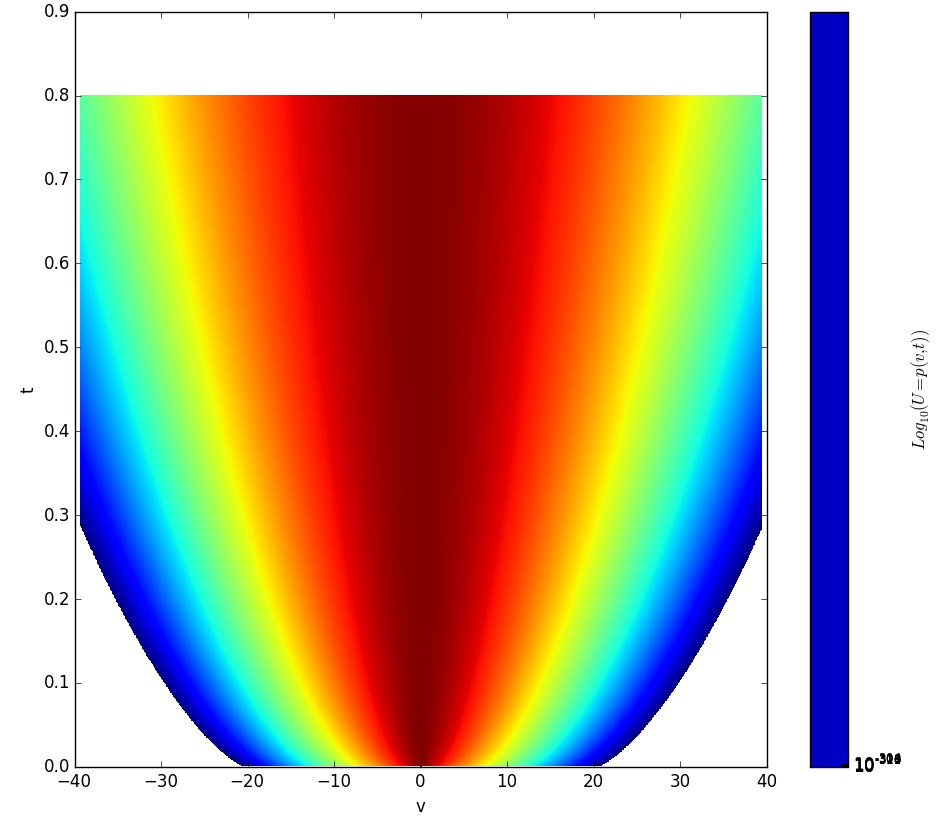
\includegraphics[scale=0.6]{figure-5-1d_planck.png}
%	\caption{Position vs. Density plot for the initial states  $\rho_L = 10, P_L = 100, v_L = 0.0$ and $\rho_R = 1.0, P_R = 1.0, v_R = 0.0$ with $\gamma = 1.4$. The initial discontinuity is at $x = 0.5$.}
%\end{figure}
% ================================================

\section*{Conclusion and Further Developments}

For 1D heat equation, the numerical solutions with the Crank Nicolson method shows qualitatively expected diffusion behavior. Moreover, Fig. 2 verified the convergence rate of 2.0 for the CN method in comparison with the analytical solution.

For 2D heat equation, the results qualitatively agree with the the behavior of heat diffusion. It was also verified, in comparison with the explicit method, that the CN method is more stable and efficient than explicit method to compute the numerical solution of 2D heat equation for higher resolution.

For further developments, (1) it is important to quantitatively inspect the convergence rate of the CN method for the 2D heat equation; and (2) develop the existing 2D heat equation into 2D Fokker-Planck equation.

\section*{Acknowledgement}
I am thankful to Goeffrey Ryan, Professor Xiao-Jing Wang, Dr. Francis Song, and Professor Andrew MacFadyen for helpful discussions and support.

% ================================================
\section*{References}
[1] R. Kiani and M. N. Shadlen, Science 324, 759 (2009). \par
[2] R. Kiani, L. Corthell, and M. N. Shadlen, Neuron 84, 1329 (2014). \par
[3] Crank-Nicolson method. Wikipedia \href{https://en.wikipedia.org/wiki/Crank-Nicolson_method}{(\textcolor{blue}{Link})} \par
[4] Alternating direction implicit method. Wikipedia \href{https://en.wikipedia.org/wiki/Alternating_direction_implicit_method}{(\textcolor{blue}{Link})} \par
[5] T. Lakoba, MATH 337, The Heat equation in 2 and 3 spatial dimensions (2016). \par
[6] G.R. Walther, The Crank Nicolson Method (2013). \href{http://georg.io/2013/12/Crank_Nicolson/} {(\textcolor{blue}{Link})}

\section*{List of Figures}
figure 1: (1D) Heat equation \\
figure 2: (1D) Heat equation \\
figure 3: (1D) $L_1$ error in heat equation (Convergence plot)\\
figure 4: (1D) Fokker-Planck equation ($p(v,t$) vs $t$) \\
figure 5: (1D) Fokker-Planck equation ($p(v,t$) vs $t$) \\
figure 6: (1D) Referenced Fokker-Planck equation ($p(v,t$) vs $t$) \\
figure 7: (2D) Heat equation with Explicit method\\
figure 8-10: (2D) Heat equation with Alternating Direction Implicit (ADI) method\\

\end{document}